% Created 2022-01-07 Fri 01:35
% Intended LaTeX compiler: pdflatex
\RequirePackage{fix-cm}
\PassOptionsToPackage{svgnames}{xcolor}
\documentclass[11pt]{article}
\usepackage{sectsty}
\allsectionsfont{\sffamily}
\usepackage{enumitem}
\setlist[description]{style=unboxed,font=\sffamily\bfseries}
\usepackage{listings}
\lstset{frame=single,aboveskip=1em,
	framesep=.5em,backgroundcolor=\color{AliceBlue},
	rulecolor=\color{LightSteelBlue},framerule=1pt}
\usepackage{xcolor}
\newcommand\basicdefault[1]{\scriptsize\color{Black}\ttfamily#1}
\usepackage{titlesec}
\newcommand{\sectionbreak}{\clearpage}
\lstset{basicstyle=\basicdefault{\spaceskip1em}}
\lstset{literate=
	    {§}{{\S}}1
	    {©}{{\raisebox{.125ex}{\copyright}\enspace}}1
	    {«}{{\guillemotleft}}1
	    {»}{{\guillemotright}}1
	    {Á}{{\'A}}1
	    {Ä}{{\"A}}1
	    {É}{{\'E}}1
	    {Í}{{\'I}}1
	    {Ó}{{\'O}}1
	    {Ö}{{\"O}}1
	    {Ú}{{\'U}}1
	    {Ü}{{\"U}}1
	    {ß}{{\ss}}2
	    {à}{{\`a}}1
	    {á}{{\'a}}1
	    {ä}{{\"a}}1
	    {é}{{\'e}}1
	    {í}{{\'i}}1
	    {ó}{{\'o}}1
	    {ö}{{\"o}}1
	    {ú}{{\'u}}1
	    {ü}{{\"u}}1
	    {¹}{{\textsuperscript1}}1
            {²}{{\textsuperscript2}}1
            {³}{{\textsuperscript3}}1
	    {ı}{{\i}}1
	    {—}{{---}}1
	    {’}{{'}}1
	    {…}{{\dots}}1
            {⮠}{{$\hookleftarrow$}}1
	    {␣}{{\textvisiblespace}}1,
	    keywordstyle=\color{DarkGreen}\bfseries,
	    identifierstyle=\color{DarkRed},
	    commentstyle=\color{Gray}\upshape,
	    stringstyle=\color{DarkBlue}\upshape,
	    emphstyle=\color{Chocolate}\upshape,
	    showstringspaces=false,
	    columns=fullflexible,
	    keepspaces=true}
\usepackage[a4paper,margin=1in,left=1.5in]{geometry}
\usepackage{parskip}
\makeatletter
\makeatother
\usepackage[utf8]{inputenc}
\usepackage[T1]{fontenc}
\usepackage{graphicx}
\usepackage{longtable}
\usepackage{wrapfig}
\usepackage{rotating}
\usepackage[normalem]{ulem}
\usepackage{amsmath}
\usepackage{amssymb}
\usepackage{capt-of}
\usepackage{hyperref}
\hypersetup{linkcolor=LightBlue,urlcolor=DarkBlue,
  citecolor=DarkRed,colorlinks=true}
\AtBeginDocument{\renewcommand{\UrlFont}{\ttfamily}}
\author{Daniel Biasiotto}
\date{\today}
\title{BD Vaccini\\\medskip
\large Progetto del Corso di Basi di Dati di Daniel Biasiotto (914117).}
\hypersetup{
 pdfauthor={Daniel Biasiotto},
 pdftitle={BD Vaccini},
 pdfkeywords={},
 pdfsubject={},
 pdfcreator={Emacs 28.0.50 (Org mode 9.6)}, 
 pdflang={English}}
\begin{document}

\maketitle
\tableofcontents


\section{Progettazione Concettuale}
\label{sec:org68b6c08}

\subsection{Requisiti Iniziali}
\label{sec:org00759ce}
Si vuole realizzare una base di dati per la gestione di una campagna vaccinale su scala
nazionale in risposta alla recente epidemia di COVID19 che ha colpito il Paese.

Ogni cittadino è un potenziale vaccinando di cui sono noti nome, cognome, età, città ed indirizzo di residenza, codice fiscale.
I cittadini sono ulteriormente suddivisibili secondo l'occupazione in personale sanitario e scolastico, categorie fragili (es, soggetti immunodepressi) e altri.

Sono disponibili tre tipi di vaccino: COVIDIN, CORONAX e FLUSTOP.
Ogni vaccino ha un'età minima e massima di somministrazione e una certa efficacia.
Ogni vaccino può richiedere una (FLUSTOP) o due (COVIDIN, CORONAX) somministrazioni. Nel caso siano necessarie due somministrazioni, l'intervallo temporale minimo tra prima e seconda dose varia da vaccino a vaccino.
Ogni vaccino è organizzato in lotti con data di produzione e scadenza. Di ogni lotto si conoscono le reazioni allergiche eventualmente riscontrate nel Paese.

I centri vaccinali sono distribuiti nelle varie città del Paese a diversi indirizzi e possono esserci più centri per ogni città;
ogni centro vaccinale dispone in ogni momento di zero o più fiale di uno o più vaccini ed a ogni centro afferiscono uno o più medici.

Ogni cittadino può fare richiesta di vaccinazione prenotando tramite un sito web o una app per smartphone (Figura 1), lasciando anche un recapito per essere ricontattati. Nel caso del sito web, é richiesto un indirizzo email al posto del numero di cellulare.

Una task force di operatori riceve le richieste di vaccinazione ed organizza un appuntamento vaccinale come segue.
Ogni cittadino vaccinando può essere indirizzato esclusivamente ad un centro localizzato nella città di residenza.
Personale sanitario e personale scolastico possono accedere ai vaccini COVIDIN e CORONAX.
I soggetti fragili possono accedere solo a CORONAX e FLUSTOP.
Gli altri soggetti non possono accedere a CORONAX.

Nel caso il cittadino abbia avuto precedenti reazioni allergiche, non può essere raccomandato nessun vaccino per cui almeno un lotto abbia registrato una segnalazione di reazione avversa negli ultimi 30 giorni.
Il cittadino viene indirizzato al centro più vicino alla residenza dove vi sia disponibilità di almeno una fiala di vaccino compatibile con i vincoli sopra.
Nel caso in cui il vaccinando abbia positività pregressa ad un test COVID, viene specificato che la seconda dose del vaccino, se prevista, non deve essere somministrata.
La persona riceve una convocazione al contatto indicato contenente data, ora, centro di vaccinazione, tipo di vaccino da somministrare.
Il cittadino vaccinando, munito di convocazione, si reca in data indicata al centro vaccinale indicato.

Ogni medico è identificato tramite i medesimi dati registrati per i cittadini, e l’afferenza ad un particolare centro vaccinale.
I medici si suddividono in medici di base e altri, dove i primi possono somministrare solo vaccini a doppia dose, mentre i secondi sono abilitati anche alla somministrazione di vaccini a singola dose.
Al momento dell’arrivo del vaccinando al centro, un medico fra quelli abilitati a somministrare il vaccino richiesto si prende in carico il vaccinando.

In seguito ad ogni vaccinazione, il medico tiene il vaccinato sotto osservazione per 15 minuti per monitorare eventuali effetti allergici relativamente al particolare lotto di vaccino utilizzato.
Se non si verificano particolari effetti avversi e il vaccino richiede un richiamo ed il soggetto non ha pregressi di positività COVID, il medico aggiorna la convocazione con un secondo appuntamento per la somministrazione presso la stessa sede dello stesso vaccino in data compatibile con le specifiche del vaccino.
Al contrario, se si verifica un effetto allergico, il medico emana un report che indica data e luogo della vaccinazione, tipo vaccino e numero lotto che hanno causato l’allergia al paziente in questione.
Il sistema deve permettere inoltre di eseguire le seguenti operazioni:
\begin{itemize}
\item Ogni sera viene stilato un rapporto che indica quante vaccinazioni sono state fatte nella giornata in tutti i centri vaccinali suddivise per categoria di cittadino.
\item Ogni sera, ogni centro vaccinale fa l’inventario del numero di dosi ancora disponibili per ogni vaccino.
\item Ogni fine settimana, viene stilato un report che indica quante vaccinazioni sono state fatte per ogni vaccino per ognuna delle categorie di cittadini e
quante di queste abbiano causato allergie
\end{itemize}

\(\pagebreak\)
\subsection{Requisiti Rivisti}
\label{sec:org773b4c0}

Si vuole realizzare una base di dati per la gestione di una campagna vaccinale su scala
nazionale in risposta alla recente epidemia di COVID19 che ha colpito il Paese.

Per i \texttt{cittadini} rappresentiamo nome, cognome, età, città, indirizzo di residenza, codice fiscale, numero di cellulare, email.
I \texttt{cittadini} possono essere personale sanitario, scolastico, categorie fragili (es. soggetti immunodepressi) e altri.

Per i \texttt{vaccini} rappresentiamo nome (COVIDIN, CORONAX e FLUSTOP), etá minima di somministrazione, etá massima di somministrazione, efficacia, numero di somministrazioni, intervallo tra dosi.

Per i \texttt{lotti} rappresentiamo il nome del vaccino, data di produzione, data di scadenza.

Per le \texttt{reazioni allergiche} rappresentiamo la reazione, il lotto, codice fiscale del cittadino.

Per i \texttt{centri vaccinali} rappresentiamo cittá, indirizzo.
Possono esserci più centri per ogni città.
Ogni \texttt{centro vaccinale} dispone in ogni momento di zero o più fiale di uno o più \texttt{vaccini}.
Ad ogni \texttt{centro vaccinale} afferiscono uno o più \texttt{medici}.

Per i \texttt{medici} rappresentiamo nome, cognome, etá, cittá, indirizzo di residenza, codice fiscale, centro vaccinale.
Ogni \texttt{medico} afferisce ad un particolare \texttt{centro vaccinale}.
I \texttt{medici} si suddividono in medici di base e altri.

Ogni \texttt{cittadino} può fare richiesta di vaccinazione prenotando tramite un sito web o una app per smartphone (Figura 1), lasciando anche un recapito per essere ricontattati. Nel caso del sito web, é richiesto un indirizzo email al posto del numero di cellulare.

Una task force di operatori riceve le richieste di vaccinazione ed organizza un appuntamento vaccinale come segue.
Ogni \texttt{cittadino} vaccinando può essere indirizzato esclusivamente ad un centro localizzato nella città di residenza.
\texttt{Personale} sanitario e personale scolastico possono accedere ai vaccini COVIDIN e CORONAX.
I \texttt{soggetti fragili} possono accedere solo a CORONAX e FLUSTOP.
Gli \texttt{altri} soggetti non possono accedere a CORONAX.

Nel caso il \texttt{cittadino} abbia avuto precedenti \texttt{reazioni allergiche}, non può essere raccomandato nessun \texttt{vaccino} per cui almeno un lotto abbia registrato una segnalazione di reazione avversa negli ultimi 30 giorni.
Il \texttt{cittadino} viene indirizzato al centro più vicino alla residenza dove vi sia disponibilità di almeno una fiala di vaccino compatibile con i vincoli sopra.
Nel caso in cui il \texttt{vaccinando} abbia positività pregressa ad un test COVID, viene specificato che la seconda dose del vaccino, se prevista, non deve essere somministrata.

La persona riceve una \texttt{convocazione} al contatto indicato contenente data, ora, centro di vaccinazione, tipo di vaccino da somministrare.
Il cittadino vaccinando, munito di convocazione, si reca in data indicata al centro vaccinale indicato.
Al momento dell’arrivo del vaccinando al centro, un medico fra quelli abilitati a somministrare il vaccino richiesto si prende in carico il vaccinando.
I medici di base possono somministrare solo vaccini a doppia dose, mentre gli altri sono abilitati anche alla somministrazione di vaccini a singola dose

\subsubsection{Glossario dei termini}
\label{sec:org0027f78}
\begin{center}
\tiny
\begin{tabular}{llll}
\textbf{termine} & \textbf{descrizione} & \textbf{sinonimi} & \textbf{collegamenti}\\
\hline
cittadino & persona residente in Italia, puó essere & vaccinando, persona, & vaccini, cittá\\
 & personale sanitario, scolastico, altro & paziente, soggetto & reazioni\\
\hline
medico & di base o altri, afferiscono ad un centro, &  & centro, cittá\\
 & amministrano le dosi dei vaccini &  & \\
\hline
vaccinazione & di un cittadino con un vaccino specifico, &  & cittadino,\\
 & con richiamo se necessario &  & vaccino\\
\hline
vaccino & COVIDIN, CORONAX o FLUSTOP &  & vaccinazione\\
\hline
convocazione & di un cittadino ad un centro vaccinale &  & vaccinazione,\\
 & per un vaccino &  & vaccino,\\
 &  &  & cittadino\\
\hline
lotto & unitá organizzativa di un vaccino, &  & reazioni allergiche,\\
 & ha una data di produzione e scadenza, &  & vaccino\\
\hline
reazione allergica & reazioni riscontrate in Italia, & reazione avversa, & cittadino, lotto\\
 & da un cittadino verso un lotto & effetti avversi, & \\
 &  & allergia & \\
\hline
centro vaccinale & centro in cui i cittadini possono vaccinarsi & centro & cittá\\
\hline
cittá & in cui si trovano i centri vaccinali & residenza & centro vaccinale,\\
 &  &  & cittadino\\
\hline
fiala & singola dose di vaccino & dose & lotto, vaccino,\\
 &  &  & centro vaccinale\\
\hline
\end{tabular}
\end{center}
\(\pagebreak\)

\subsection{Schema ER Iniziale}
\label{sec:orgd477f49}
\begin{center}
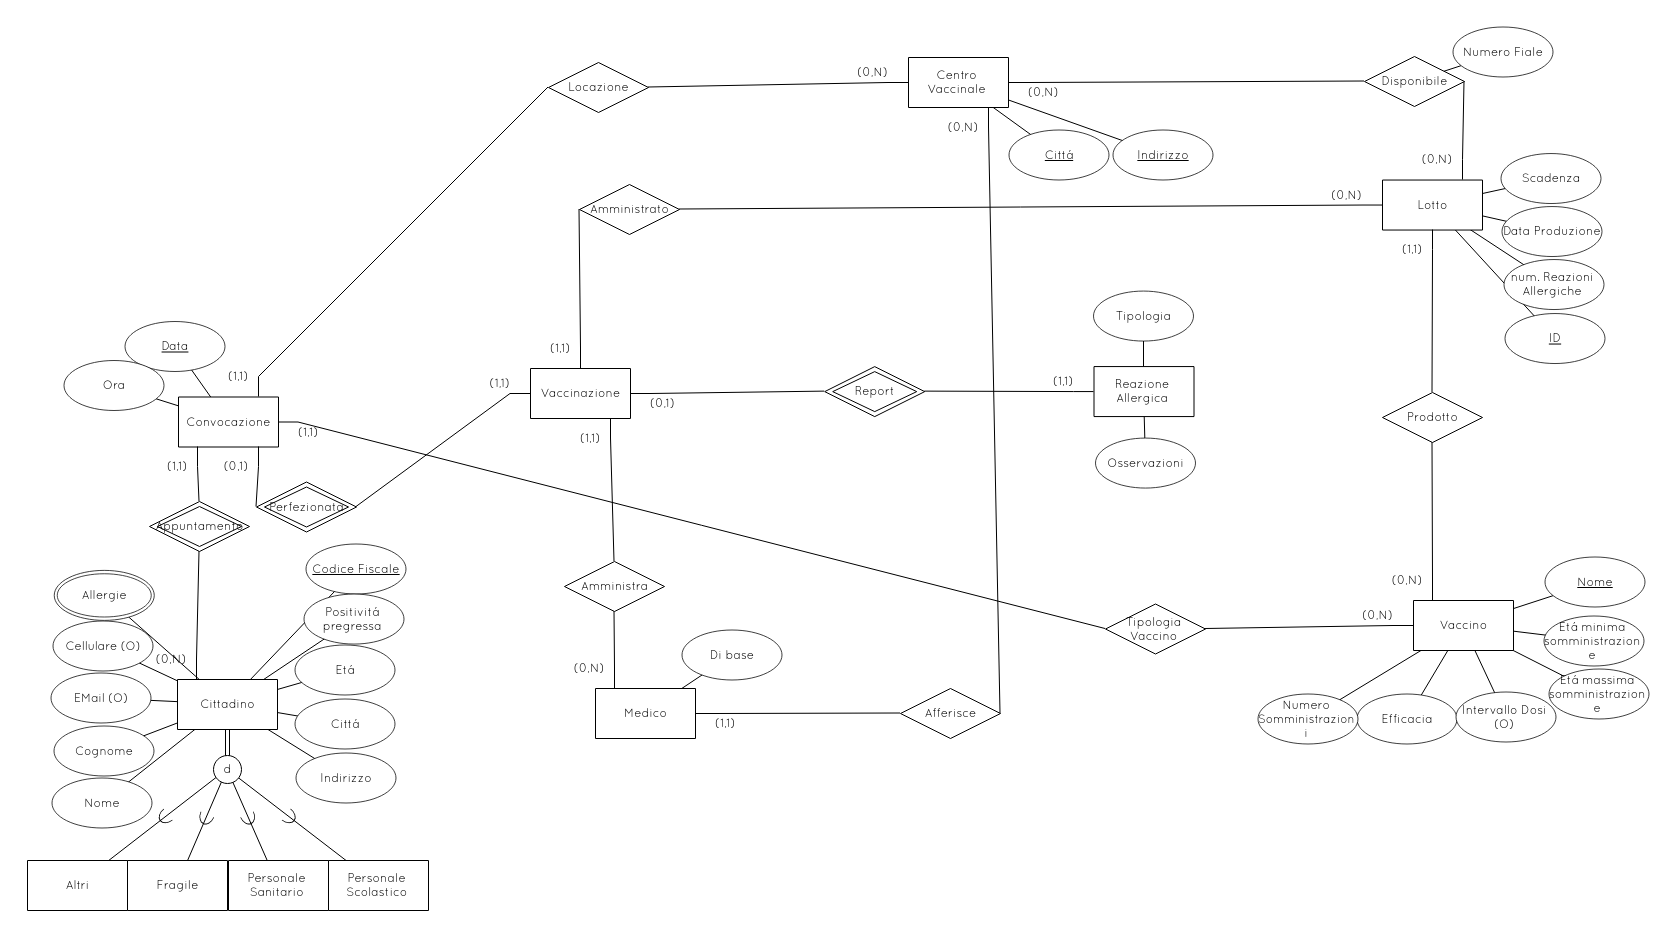
\includegraphics[width=.9\linewidth]{/home/dnbias/Uni/II/BD/Progetto/Schema ER - Concettuale.png}
\end{center}
\subsection{Business Rules}
\label{sec:orgf818be1}
\begin{itemize}
\item Un \texttt{cittadino} puó accedere solo a centri vaccinali della propria cittá di residenza
\item Un \texttt{cittadino} per un dato \texttt{vaccino} deve al massimo avere confermato \(n\) appuntamenti con \(n\) uguale al Numero Somministrazioni del Vaccino
\item Un \texttt{cittadino} per poter ricevere un \texttt{vaccino} deve avere Etá compresa tra le etá minima e massima di somministrazione
\item Un \texttt{cittadino} deve ricevere un dato \texttt{vaccino} in base alla propria categorizzazione:
\begin{itemize}
\item fragile, \texttt{CORONAX}, \texttt{FLUSTOP}
\item personale sanitario, \texttt{COVIDIN}, \texttt{CORONAX}
\item personale scolastico, \texttt{COVIDIN}, \texttt{CORONAX}
\item nessuno dei precedenti, \texttt{CORONAX}
\end{itemize}
\item Un \texttt{cittadino} che ha riscontrato \texttt{reazioni avverse} non puó accedere a dosi il  cui lotto ha riscontrato almeno una reazione avversa negli ultimi 30 giorni
\item Un \texttt{cittadino} con positivitá pregressa non deve ricevere seconda dose se specificata
\item \texttt{Medici di base} somministrano solo vaccini a doppia dose
\item Il \texttt{numero di somministrazioni} del singolo \texttt{vaccino} va aggiornato a fine giornata in base agli appuntamenti che non sono stati annullati
\item Il \texttt{numero di fiale disponibili} per ogni lotto di cui dispone un \texttt{centro vaccinale} va tenuto aggiornato in base alle vaccinazione fatte
\end{itemize}

\subsection{Schema + BR}
\label{sec:org81a53a8}

\section{Progettazione Logica}
\label{sec:orgbc06cd7}

\subsection{Tavola dei Volumi}
\label{sec:org7c40d58}
\begin{center}
\begin{tabular}{llr}
Concetto & Tipo & Volume\\
\hline
Cittadino & E & 60000000\\
Fragile & E & 5000000\\
Personale Sanitario & E & 800000\\
Personale Scolastico & E & 1000000\\
Altri & E & 55200000\\
Medico & E & 400000\\
Vaccino & E & 3\\
Lotto & E & 2000\\
Centro Vaccinale & E & 8000\\
Reazione Allergica & E & 1000\\
Vaccinazione & E & 20000000\\
Convocazione & E & 21000000\\
Appuntamento & A & 21000000\\
Incarico & A & 400000\\
Reazione & A & 1000\\
Locazione & A & 20000000\\
Amministra & A & 20000000\\
Afferisce & A & 400000\\
Disponibile & A & 24000\\
Prodotto & A & 2000\\
\hline
\end{tabular}
\end{center}

Giustificazioni per i volumi
\begin{itemize}
\item Approssimazione Cittadini in Italia
\begin{itemize}
\item Sottoinsiemi dei Cittadini stimati in base al numero di Cittadini e Medici
\end{itemize}
\item Approssimazione Medici in Italia
\item Numero Vaccini dai requisiti
\item Approssimazione Lotti in assenza di dati
\item Centri vaccinali in base ai comuni italiani
\item Reazioni allergiche in base ai dati
\item Vaccinazioni supponendo base dati nel corso della campagna vaccinale
\item Convocazioni supponendole maggiori delle Vaccinazioni
\item Appuntamenti, in base al numero di Convocazioni
\item Incarichi in base al numero di Medici
\item Reazioni in base al numero di Reazioni allergiche
\item Locazioni in base al numero di Vaccinazioni
\item Amministrazioni in base al numero di Vaccinazioni
\item Afferisce, in base al numero di Medici
\item Disponibile, supponendo almeno 3 lotti diversi per ogni Centro Vaccinale
\item Prodotto, in base al numero di lotti
\end{itemize}

\subsection{Tavola delle Operazioni}
\label{sec:org5c1831e}
\begin{center}
\begin{tabular}{rlll}
Operazione & Descrizione & Tipo & Frequenza\\
\hline
1 & Rapporto delle vaccinazioni della giornata & B & 1 al giorno\\
 & in tutti i centri vaccinali &  & \\
 & suddivise per categoria di cittadino &  & \\
\hline
2 & Inventario del numero di dosi disponibili & B & 1 al giorno\\
 & per ogni vaccino di un dato centro vaccinale &  & \\
\hline
3 & Rapporto delle vaccinazioni per ogni vaccino & B & 1 a settimana\\
 & per ognuna delle categorie di cittadini &  & \\
 & e quante di queste abbiano causato &  & \\
 & reazioni allergiche &  & \\
\hline
4 & Aggiunta di un Cittadino & I & 80000 al giorno\\
\hline
5 & Aggiunta di una Convocazione & I & 120000 al giorno\\
\hline
6 & Aggiunta di una Vaccinazione & I & 100000 al giorno\\
\hline
7 & Aggiunta di un Lotto & I & 2 a settimana\\
\hline
8 & Aggiunta di un Medico & I & 2 a settimana\\
\hline
9 & Inserimento di una Reazione Allergica ad & I & 3 a settimana\\
 & una vaccinazione (Report) &  & \\
\hline
\end{tabular}
\end{center}


\(\pagebreak\)
\subsection{Analisi delle Ridondanze}
\label{sec:org4e1143a}
\begin{itemize}
\item Ridondanza: \texttt{reazioni allergiche} verso un lotto come attributo dello stesso
\begin{itemize}
\item impatta le operazioni \texttt{3}, \texttt{9}
\end{itemize}
\end{itemize}

\subsubsection{Operazione 3}
\label{sec:orgfff760e}
\begin{enumerate}
\item Con Ridondanza
\label{sec:orgd8a03f4}

Lo schema di visita é:
\texttt{Vaccinazione} - \texttt{Perfezionata} - \texttt{Convocazione} - \texttt{Appuntamento}
\begin{itemize}
\item \texttt{Cittadino} - \texttt{Fragile} - \texttt{Personale Scolastico} - \texttt{Personale Sanitario} - \texttt{Altri}
\item \texttt{Vaccino} - \texttt{Prodotto} - \texttt{Lotto}
\end{itemize}

La tavola degli accessi é:
\begin{center}
\begin{tabular}{llll}
Concetto & Costrutto & Accessi & Tipo\\
\hline
Vaccinazione & E & 20M & L\\
Perfezionata & A & 20M & L\\
Convocazione & E & 20M & L\\
Appuntamento & A & 20M & L\\
Cittadino & E & 20M & L\\
Fragile & E & 1,66M & L\\
Personale Scolastico & E & 260K & L\\
Personale Sanitario & E & 320K & L\\
Altri & E & 17,76M & L\\
Vaccino & E & 3 & L\\
Prodotto & A & 2000 & L\\
Lotto & E & 2000 & L\\
\end{tabular}
\end{center}

Dove:
\begin{itemize}
\item \texttt{Fragili} sono l'8.3\% dei \texttt{Cittadini}
\item \texttt{Personale Sanitario} sono l'1.3\% dei \texttt{Cittadini}
\item \texttt{Personale Scolastico} sono l'1.6\% dei \texttt{Cittadini}
\item \texttt{Altri} sono l'88.8\% dei \texttt{Cittadini}
\end{itemize}

Accessi Totali: 120'004'003 in Lettura

\item Senza Ridondanza
\label{sec:org321e015}

Lo schema di visita é:
\texttt{Vaccinazione} - \texttt{Perfezionata} - \texttt{Convocazione} - \texttt{Appuntamento}
\begin{itemize}
\item \texttt{Cittadino} - \texttt{Fragile} - \texttt{Personale Scolastico} - \texttt{Personale Sanitario} - \texttt{Altri}
\item \texttt{Report} - \texttt{Reazione Allergica} - \texttt{Tipologia Vaccino} - \texttt{Vaccino}
\end{itemize}

La tavola degli accessi é:
\begin{center}
\begin{tabular}{llll}
Concetto & Costrutto & Accessi & Tipo\\
\hline
Vaccinazione & E & 20M & L\\
Perfezionata & A & 20M & L\\
Convocazione & E & 20M & L\\
Appuntamento & A & 20M & L\\
Cittadino & E & 20M & L\\
Fragile & E & 1,66M & L\\
Personale Scolastico & E & 260K & L\\
Personale Sanitario & E & 320K & L\\
Altri & E & 17,76M & L\\
Report & A & 320 & L\\
Reazione Allergica & A & 320 & L\\
Tipologia Vaccino & E & 20M & L\\
Vaccino & E & 20M & L\\
\end{tabular}
\end{center}

Dove valgono le considerazioni precedenti e:
\begin{itemize}
\item \texttt{Report} sono \[\frac{1000}{20000000} = 0.00005\%\] delle \texttt{Vaccinazioni}
\end{itemize}

Accessi Totali: 160'000'640 in Lettura

\(\pagebreak\)
\end{enumerate}
\subsubsection{Operazione 9}
\label{sec:org5b660b9}
\begin{enumerate}
\item Con Ridondanza
\label{sec:orga14ef69}

Lo schema di visita é:
\texttt{Reazione Allergica} - \texttt{Report} - \texttt{Vaccinazione} - \texttt{Amministrato} - \texttt{Lotto}

\begin{center}
\begin{tabular}{llrl}
Concetto & Costrutto & Accessi & Tipo\\
\hline
Reazione Allergica & E & 1 & S\\
Report & A & 1 & S\\
Vaccinazione & E & 1 & L\\
Amministrato & A & 1 & L\\
Lotto & E & 1 & S\\
\end{tabular}
\end{center}


Accessi Totali: 8 (Supponendo gli accessi in scrittura equivalenti a 2 accessi in lettura)

\item Senza Ridondanza
\label{sec:org16862af}

Lo schema di visita é:
\texttt{Reazione Allergica} - \texttt{Report}
\begin{center}
\begin{tabular}{llrl}
Concetto & Costrutto & Accessi & Tipo\\
\hline
Reazione Allergica & E & 1 & S\\
Report & A & 1 & S\\
\end{tabular}
\end{center}

Accessi Totali: 4
\(\pagebreak\)
\end{enumerate}
\subsubsection{Analisi}
\label{sec:org555965f}
Presenza di Ridondanza:
\begin{itemize}
\item Spazio: \[4 \text{ byte} \times 2000 = 8000 \text{ byte}\]
\item Tempo:
\begin{itemize}
\item Operazione 3 - \[120004003 \text{ accessi} \times 1 \text{ volta a settimana}\]
\item Operazione 9 - \[8 \text{ accessi} \times 3 \text{ volte a settimana}\]
\item Totale - \[120004027 \text{ accessi a settimana}\]
\end{itemize}
\end{itemize}

Assenza di Ridondanza:
\begin{itemize}
\item Spazio: \[0 \text{ byte} \times 2000 = 0 \text{ byte}\]
\item Tempo:
\begin{itemize}
\item Operazione 3 - \[160000640 \text{ accessi} \times 1 \text{ volta a settimana}\]
\item Operazione 9 - \[4 \text{ accessi} \times 3 \text{ volte a settimana}\]
\item Totale - \[160000652 \text{ accessi a settimana}\]
\end{itemize}
\end{itemize}

Scegliamo di tenere la ridondanza a fronte del risparmio di quasi 40 milioni di accessi con l'utilizzo di solo 8000 byte.

\subsection{Schema ER Ristrutturato \& Business Rules}
\label{sec:org745cd07}
\begin{center}
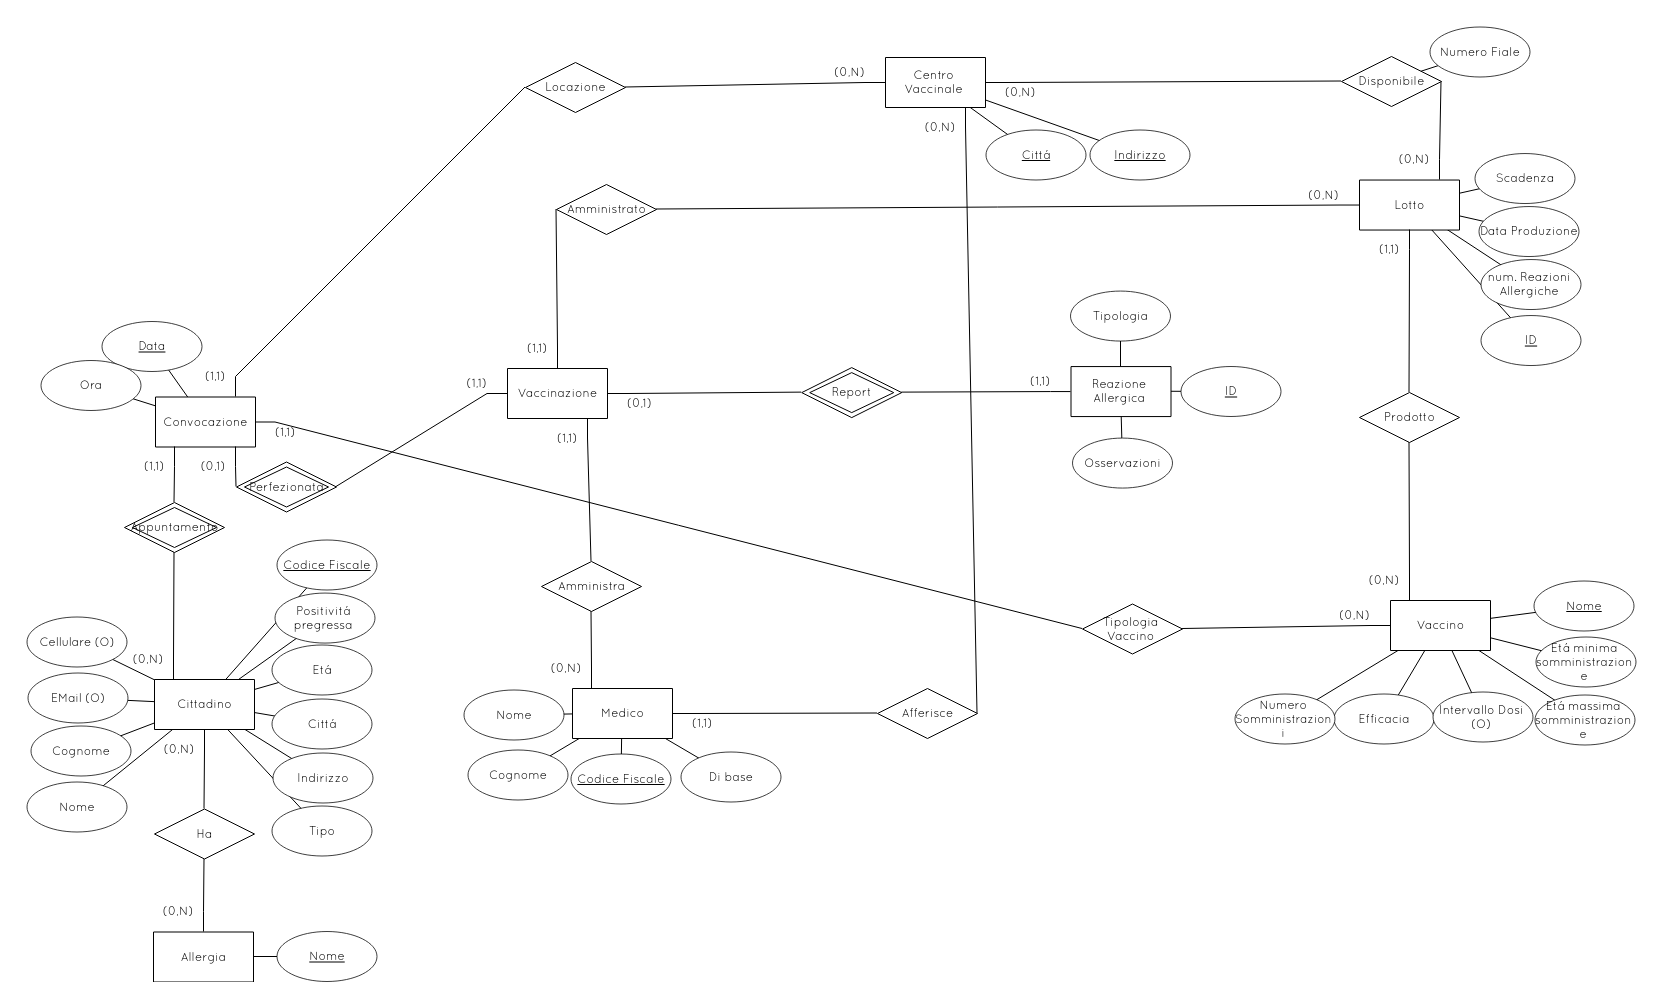
\includegraphics[width=.9\linewidth]{/home/dnbias/Uni/II/BD/Progetto/Schema ER - Ristrutturato.png}
\end{center}

Regole Aziendali:
\begin{itemize}
\item Un \texttt{cittadino} puó accedere solo a centri vaccinali della propria cittá di residenza
\item Un \texttt{cittadino} per un dato \texttt{vaccino} deve al massimo avere confermato \(n\) appuntamenti con \(n\) uguale al Numero Somministrazioni del Vaccino
\item Un \texttt{cittadino} per poter ricevere un \texttt{vaccino} deve avere Etá compresa tra le etá minima e massima di somministrazione
\item Un \texttt{cittadino} deve ricevere un dato \texttt{vaccino} in base alla propria categorizzazione:
\begin{itemize}
\item fragile, \texttt{CORONAX}, \texttt{FLUSTOP}
\item personale sanitario, \texttt{COVIDIN}, \texttt{CORONAX}
\item personale scolastico, \texttt{COVIDIN}, \texttt{CORONAX}
\item nessuno dei precedenti, \texttt{CORONAX}
\end{itemize}
\item Un \texttt{cittadino} che ha riscontrato \texttt{reazioni avverse} non puó accedere a dosi il cui lotto ha riscontrato almeno una reazione avversa negli ultimi 30 giorni
\item Un \texttt{cittadino} con positivitá pregressa non deve ricevere seconda dose se specificata
\item \texttt{Medici di base} somministrano solo vaccini a doppia dose
\item Il \texttt{numero di fiale disponibili} per ogni lotto di cui dispone un \texttt{centro vaccinale} va tenuto aggiornato in base alle vaccinazione fatte
\item Il \texttt{tipo} di un \texttt{cittadino} deve corrispondere ad una categorizzazione: fragile, personale sanitario, personale scolastico, altro
\end{itemize}

L'attributo multivalore \texttt{Allergia} é stato convertito nella relazione molti a molti \texttt{Ha} e nell'entitá \texttt{Allergia}
La generalizzazione totale/esclusiva  di \texttt{Cittadino} é stata convertita del attributo \texttt{Tipo} dello stesso

\subsection{Schema Relazionale}
\label{sec:orgb188241}
Vaccino( \uline{Nome}, EtáMinima, EtáMassima,
            IntervalloDosi*, Efficacia, NumSomministrazioni)

Lotto( \uline{ID}, NomeVaccino, NumReazioniAllergiche, DataProduzione, Scadenza)

CentroVaccinale( \uline{Cittá}, \uline{Indirizzo})

Disponibile( \uline{Cittá}, \uline{Indirizzo}, \uline{Lotto}, NumFiale)

Convocazione( \uline{Data}, \uline{CodiceFiscale}, Cittá, Indirizzo, Ora)

Cittadino( \uline{CodiceFiscale}, Etá, Nome, Cognome, Cittá, Indirizzo,
               EMail*,PositivitáPregressa, Cellulare*, Tipo)

Allergia( \uline{Nome})

Ha( \uline{CodiceFiscale}, \uline{Allergia})

Vaccinazione( \uline{CodiceFiscale}, \uline{Data}, CodiceFiscaleMedico, ID)

Medico( \uline{CodiceFiscale}, Cittá, Indirizzo, Nome, Cognome, Di Base)

ReazioneAllergica( \uline{ID} ,Tipologia, Osservazioni, CodiceFiscale, Data)

\(\\\)

Lotto(NomeVaccino) \emph{referenzia} Vaccino(Nome)

Disponibile(Cittá, Indirizzo) \emph{referenzia} CentroVaccinale(Cittá, Indirizzo)

Disponibile(Lotto) \emph{referenzia} Lotto(ID)

Convocazione(CodiceFiscale) \emph{referenzia} Cittadino(CodiceFiscale)

Convocazione(Cittá, Indirizzo) \emph{referenzia} CentroVaccinale(Cittá, Indirizzo)

Ha(Codice Fiscale) \emph{referenzia} Cittadino(CodiceFiscale)

Ha(Allergia) \emph{referenzia} Allergia(Nome)

Medico(Cittá, Indirizzo) \emph{referenzia} CentroVaccinale(Cittá, Indirizzo)

Vaccinazione(Codice Fiscale, Data) \emph{referenzia} Convocazione(CodiceFiscale, Data)

ReazioneAllergica(CodiceFiscale, Data) \emph{referenzia} Vaccinazione(CodiceFiscale, Data)

\(\pagebreak\)
\section{Implementazione}
\label{sec:orgd6afdcd}
\subsection{DDL}
\label{sec:orgeb33f87}
\lstset{language=SQL,label= ,caption= ,captionpos=b,numbers=none}
\begin{lstlisting}
DROP SCHEMA "BDvaccini" cascade;

CREATE SCHEMA "BDvaccini" AUTHORIZATION dbdanielbiasiotto;

CREATE TABLE Vaccino(
         Nome varchar(20) primary key,
         EtáMinima smallint default 0 not null,
         EtáMassima smallint default 100 not null,
         IntervalloDosi smallint not null,
         Efficacia float not null,
         NumSomministrazioni smallint not null
       );
CREATE TABLE Lotto(
         ID SERIAL primary key,
         NomeVaccino varchar(20),
         NumReazioniAllergiche smallint default 0 not null,
         DataProduzione date not null,
         Scadenza date not null,
         constraint fk_lotto
            foreign key(NomeVaccino)
                references Vaccino(Nome)
                    on update cascade
                    on delete cascade
       );
CREATE TABLE CentroVaccinale(
         Cittá varchar(30),
         Indirizzo varchar(50),
         primary key(Cittá, Indirizzo)
       );
CREATE TABLE Medico(
         CodiceFiscale char(16) primary key,
         Cittá varchar(30),
         Indirizzo varchar(50),
         Nome varchar(20) not null,
         Cognome varchar(20) not null,
         DiBase boolean default true not null,
         constraint fk_medico
            foreign key(Cittá, Indirizzo)
                references CentroVaccinale(Cittá, Indirizzo)
                    on update cascade
                    on delete cascade
       );
CREATE TABLE Disponibile(
         Cittá varchar(30),
         Indirizzo varchar(50),
         Lotto smallint,
         NumFiale smallint not null,
         primary key(Cittá, Indirizzo, Lotto),
         constraint fk_disponibile
             foreign key(Cittá, Indirizzo)
                 references CentroVaccinale(Cittá, Indirizzo),
             foreign key(Lotto)
                 references Lotto(ID)
                     on update cascade
                     on delete cascade
       );
CREATE TABLE Cittadino(
         CodiceFiscale char(16) primary key,
         Etá smallint not null,
         Nome varchar(20) not null,
         Cognome varchar(20) not null,
         Cittá varchar(20) not null,
         Indirizzo varchar(20) not null,
         Email varchar(30),
         Cellulare varchar(10),
         Tipo varchar(20) default 'altro' not null,
         PositivitáPregressa boolean default false not null,
         unique(Nome, Cognome, Cittá)
       );
CREATE TABLE Convocazione(
         Data date,
         CodiceFiscale char(16),
         Cittá varchar(30),
         Indirizzo varchar(50),
         Ora time not null,
         primary key(Data, CodiceFiscale),
         constraint fk_convocazione
             foreign key(CodiceFiscale)
                 references Cittadino(CodiceFiscale)
                     on update cascade
                     on delete cascade,
             foreign key(Cittá, Indirizzo)
                 references CentroVaccinale(Cittá, Indirizzo)
                     on update cascade
                     on delete cascade
       );

CREATE TABLE Allergia(
         Nome varchar(30) primary key
       );
CREATE TABLE Ha(
         CodiceFiscale char(16),
         Allergia varchar(30),
         primary key(CodiceFiscale, Allergia),
         constraint fk_ha
             foreign key(CodiceFiscale)
                 references Cittadino(CodiceFiscale)
                     on update cascade
                     on delete cascade,
         foreign key(Allergia)
             references Allergia(Nome)
                 on update cascade
                 on delete cascade
       );
CREATE TABLE Vaccinazione(
         Data date,
         CodiceFiscale char(16),
         CodiceFiscaleMedico char(16),
         ID smallint,
         primary key(CodiceFiscale,Data),
         constraint fk_vaccinazione
             foreign key(CodiceFiscale, Data)
                 references Convocazione(CodiceFiscale, Data)
                     on update cascade
                     on delete cascade,
             foreign key(CodiceFiscaleMedico)
                 references Medico(CodiceFiscale)
                     on update cascade
                     on delete cascade,
             foreign key(ID)
                 references Lotto(ID)
                     on update cascade
                     on delete cascade
       );

CREATE TABLE ReazioneAllergica(
         ID smallint,
         Tipologia varchar(30) not null,
         Osservazioni varchar(500) not null,
         CodiceFiscale char(16),
         Data date,
         primary key(ID),
         constraint fk_reazione
             foreign key(ID)
                 references Lotto(ID)
                     on update cascade
                     on delete cascade,
              foreign key(CodiceFiscale, Data)
                  references Vaccinazione(CodiceFiscale, Data)
                      on update cascade
                      on delete cascade
       );

\end{lstlisting}
\(\pagebreak\)
\subsection{DML}
\label{sec:org9a26ab7}
\lstset{language=SQL,label= ,caption= ,captionpos=b,numbers=none}
\begin{lstlisting}
insert into "BDvaccini".vaccino values
	('Coronax', 16, 80, 6, 0.9, 2),
	('Covidin', 13, 70, 8, 0.88, 1),
	('Modernum', 20, 60, 4, 0.92, 2);

insert into "BDvaccini".cittadino values
	('BSTED23DGC23DT3C',40,'Giuseppe','Pizza',
    'Milano','Via P 17','etndduen@uen.it',387438457,
    'fragile',false),
	('CSTEEU3DGC256H3C',40,'Silvia','Enne',
    'Milano','Via Cile 1','yi@uen.it',374691923,
    'personale sanitario',false),
	('HIERR9GC287E9E8T',40,'Giusi','Emme','Piolo',
    'Via Guille 3','tieun@uen.en',387438457,
    'altro',true),
	('EUT923DGC287IET8',40,'Tito','Pi',
    'Padova','Via Maria 14b','ueioe@edu.uk',983746192,
    'personale medico',false);

insert into "BDvaccini".centrovaccinale values
	('Milano','Via Beccaria 3'),
	('Pisa','Via Venezia 12c'),
	('Torino','Via Umberto 50');

insert into "BDvaccini".lotto values
	(nextval('"BDvaccini".lotto_id_seq'::regclass),
    'Coronax', 0, '12/09/2020', '12/09/2022'),
	(nextval('"BDvaccini".lotto_id_seq'::regclass),
    'Coronax', 0, '8/02/2020', '10/02/2023'),
	(nextval('"BDvaccini".lotto_id_seq'::regclass),
    'Covidin', 0, '1/10/2020', '12/10/2021'),
	(nextval('"BDvaccini".lotto_id_seq'::regclass),
    'Modernum', 0, '12/20/2019', '12/20/2022');

insert into "BDvaccini".disponibile values
	('Milano','Via Beccaria 3',2,20),
	('Milano','Via Beccaria 3',4,200),
	('Pisa','Via Venezia 12c',2,140),
	('Torino','Via Umberto 50',3,10);

insert into "BDvaccini".allergia values
	('Albicocche');

insert into "BDvaccini".ha values
	('BSTED23DGC23DT3C','Albicocche');

insert into "BDvaccini".medico values
	('BEGIED23DGC23DT3', 'Torino', 'Via Umberto 50',
    'Harry', 'Oliver', false),
	('GITIED23DGC23DT3', 'Pisa', 'Via Venezia 12c',
    'Carla', 'Ronda', true);

insert into "BDvaccini".convocazione values
	('02/13/2020','EUT923DGC287IET8','Torino','Via Umberto 50','12:00:00'),
	('04/23/2020','BSTED23DGC23DT3C','Pisa','Via Venezia 12c','16:30:00');

insert into "BDvaccini".vaccinazione values
	('02/13/2020','EUT923DGC287IET8','BEGIED23DGC23DT3',3);

insert into "BDvaccini".reazioneallergica values
	(3,'Rossore','Lorem Ipsum','EUT923DGC287IET8','02/13/2020');
\end{lstlisting}
\subsection{Operazioni}
\label{sec:orgfd6c104}
\end{document}
